\chapter{Introdução Teórica}

Não é possível entrar no tema \textbf{Meio Ambiente} sem mencionar a Educação Ambiental nas escolas, uma vez que esperamos que nossas crianças evoluam com uma mentalidade melhor que a nossa no tocante ao meio ambiente.\\

\citeaa{Dias1994}  diz que a "Educação Ambiental se caracteriza por
incorporar as dimensões sociais, políticas, econômicas,
culturais, ecológicas e éticas, deixando claro que ao discutir
qualquer problema ambiental é fundamental a consideração
de todos estes aspectos." Segundo este autor, "a maior parte
dos problemas ambientais tem suas raízes na miséria que,
por sua vez, é gerada por políticas e problemas econômicos,
concentradores de riqueza e responsáveis pelo desemprego
e degradação ambiental."\\

Pode-se também definir a educação ambiental, nas palavras de \citeonline{Magalhaes2018}, como um processo
onde o educando obtém conhecimentos acerca das
questões ambientais e assim passa a ter um novo
entendimento acerca do meio ambiente, se tornando um
agente transformador referente à preservação do meio
ambiente e de seus recursos naturais. \\

\citeaa{Gadotti2000} explica que educação ambiental vai muito além do conservacionismo
Trata-se de uma mudança radical de mentalidade em
relação à qualidade de vida, que está diretamente ligada
ao tipo de convivência que mantemos com a natureza e
que implica em atitudes, valores, ações. Trata-se de uma
opção de vida por uma relação saudável e equilibrada,
com o contexto, com os outros, com o ambiente mais
próximo, a começar pelo ambiente de trabalho e
doméstico.\\

\section{Contexto Geográfico: Brasília}

De acordo com a \citeaa{WikiPediaBrasilia20200518} A cidade começou a ser planejada e desenvolvida em 1956 por Lúcio Costa, pelo também arquiteto Oscar Niemeyer e pelo engenheiro estrutural Joaquim Cardozo. Inaugurada em 21 de abril de 1960, pelo então presidente Juscelino Kubitschek, Brasília tornou-se formalmente a terceira capital do Brasil, após Salvador e Rio de Janeiro. Vista de cima, a principal área da cidade é descrita frequentemente como tendo o formato de um avião, mas a proposta inicial de Lúcio Costa era de que se assemelhasse ao sinal da cruz, e um dos eixos foi depois arqueado para se adaptar ao relevo da região.\\

O ritmo de crescimento populacional na primeira década foi de 14,4\% ao ano, com um aumento populacional de 285\%. Na década de 1970, o crescimento médio anual foi de 8,1\%, com um incremento total de 115,52\%. A população total do Distrito Federal, que não deveria ultrapassar 500 000 habitantes em 2000, atingiu esta cota no início da década de 1970, e, entre 1980 e 1991, a população expandiu em mais 32,8\%. O Plano Piloto, que, na inauguração, concentrava 48\% da população do Distrito Federal, gradativamente perdeu importância relativa, chegando a 13,26\% em 1991, passando o predomínio para as cidades-satélite.[49]

Em 2010, o Instituto Brasileiro de Geografia e Estatística indicou 2.570.160 habitantes em todo o Distrito Federal. O Índice de Desenvolvimento Humano é de 0,824 e a taxa de analfabetismo de apenas 4,35\%. Brasília também caracteriza-se pela sua desigualdade social, sendo a quarta área metropolitana mais desigual do Brasil e a décima sexta do mundo, segundo um relatório divulgado pela Organização das Nações Unidas. \\

A população brasiliense é formada por migrantes de todas as regiões brasileiras, sobretudo do Nordeste e do Sudeste, além de estrangeiros que trabalham nas embaixadas espalhadas pela capital. Dados de 2010 apontavam que quase metade da população não nasceu ali, sendo que 1.380.873 (53,73\%) eram brasilienses e 1.189.287 (46,27\%) de outros locais (incluindo 8 577 estrangeiros, ou 0,33\% da população), principalmente de Goiás, Minas Gerais e Bahia.

A região administrativa de Brasília, composta em sua parte urbana pelos bairros residenciais Asa Norte, Asa Sul e Vila Planalto, conta com uma população de 209 855 habitantes (2010) e uma área de 472,12 km², sendo a terceira maior região administrativa do Distrito Federal em termos de população, atrás apenas de Ceilândia (com 402 729 habitantes) e Taguatinga (361 063).

\begin{figure}[h]
    \centering
    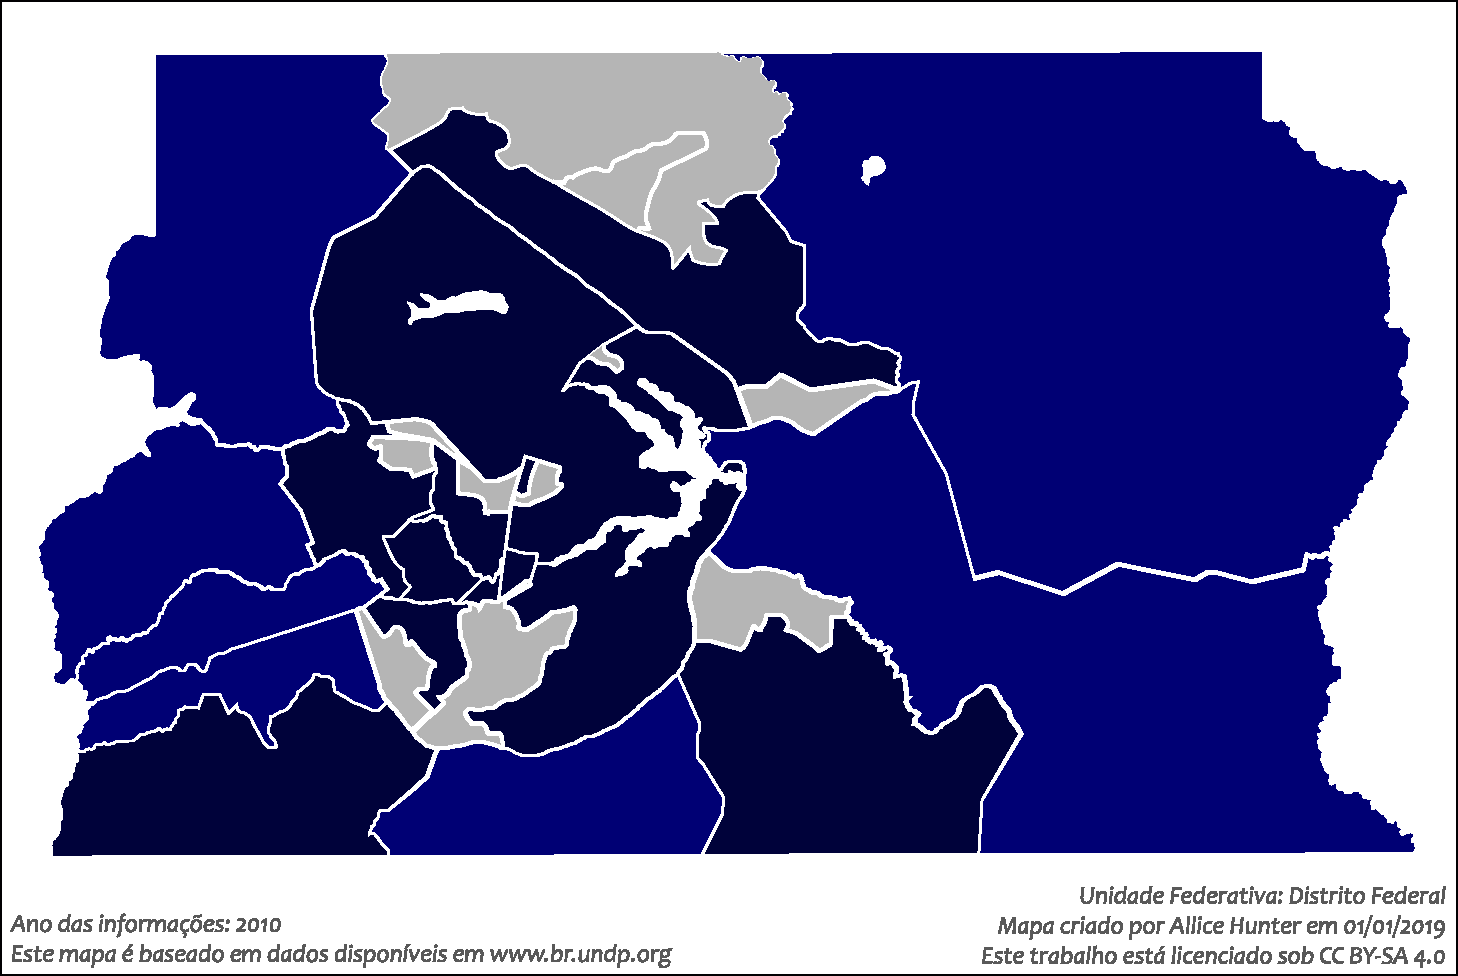
\includegraphics[width=0.9\linewidth]{2-caps/cap02/Mapa_do_IDH_do_Distrito_Federal_(2010)}
    \caption{}
    \label{fig:mapadoidhdodistritofederal2010}
\end{figure}


%\newacronym{CODEPLAN}{CODEPLAN}{Companhia de Planejamento do Distrito Federal}

De acordo com o \citeaa{CODEPLANSEPLAN2013}

\begin{figure}[h]
    \centering
    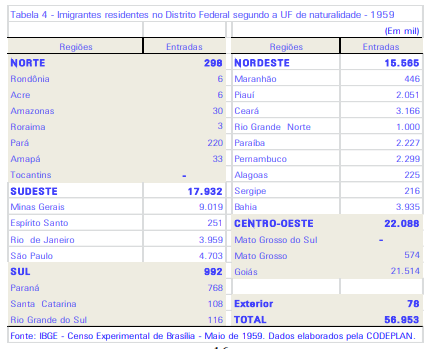
\includegraphics[width=0.7\linewidth]{fig/imigrantes-1959}
    \label{fig:imigrantes-1959}
    \caption{Imigrantes residentes no DF em 1959}
\end{figure}

\begin{figure}[h]
    \centering
    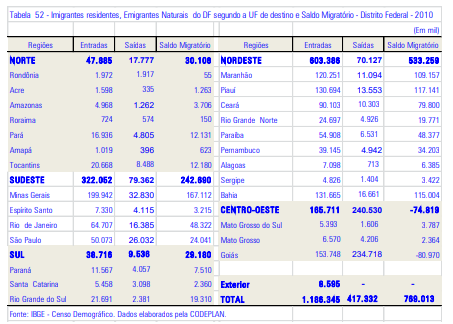
\includegraphics[width=0.7\linewidth]{fig/imigrantes-2010}
    \caption{}
    \label{fig:imigrantes-2010}
\end{figure}
